\section{Discussion}
\subsection{CPU usage and load handling stability}
The results, as depicted in fig. \ref{fig_mean_values}, show an almost linear increase in the CPU usage mean value in the Go implementation, while the multi-process C implementation considerably decreases its CPU utilization after 16 concurrent connections. Overall, the C implementation handles the load more efficiently at all levels of concurrent connections. The results might seem counter-intuitive and baffling at first glance, since many literature sources warn against the performance penalties incurred by handling context-switches in kernel-space \cite{Cox-Buday2017}\cite{Kerrisk2010}. 

Nonetheless, in a comparison based on programs similar to real-life deployed network applications, like in these experiments, the CPU usage is influenced not only by the context-switches, but also by inherent traits of the platform running the application. In this case, the actual performance gains attributable to user-space context-switching might be too small compared to the overhead of the Go runtime and the periodic garbage collection it performs.

Moreover, the CPU usage of the non-preemptively scheduled implementation has an overall higher coefficient of variation ($C_v$), calculated by dividing the standard deviation ($\sigma$) of a measurement by its mean value ($\mu$). This value allows us to answer RQ2 and compare the stability of the CPU usage of both platforms, a higher $C_v$ implies that the data points of a measurement were on average spread farther from the mean value as a measurement with a lower $C_v$. Specially over higher loads, as can be seen in fig. \ref{fig_cv}, the multi-process implementation achieves a more stable CPU utilization, which does not oscillate so far from the mean value as the Go implementation. This insight in the stability of the CPU usage of a particular paradigm has relevance to servers that periodically work close to the maximum CPU usage during high load periods, since an application with a smaller $C_v$ will react more predictably and securely close to the maximum CPU usage of a platform.

\begin{figure}[h]
	\centering
	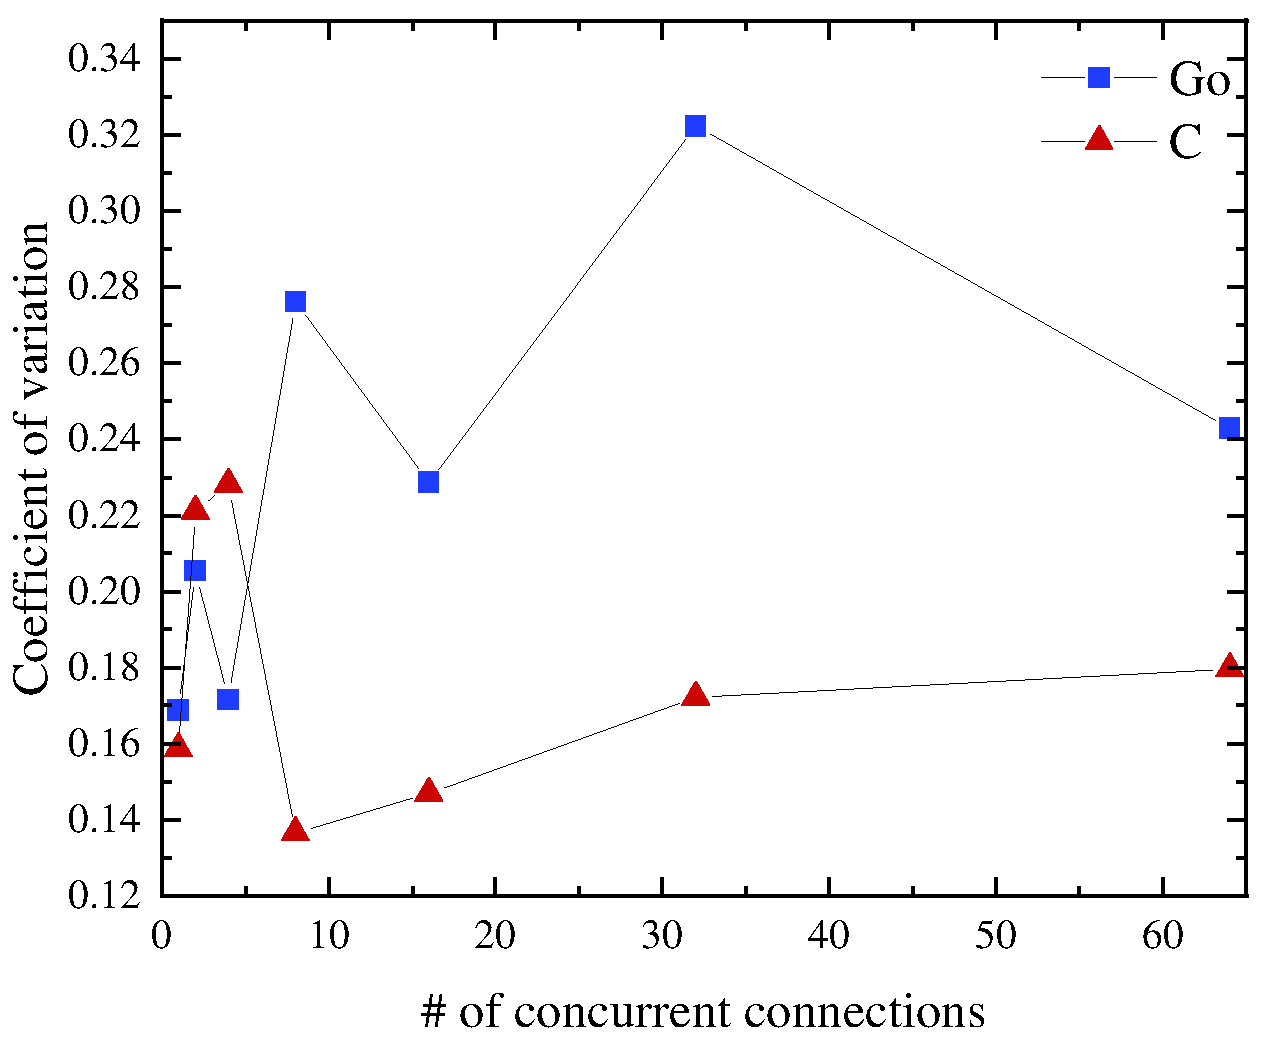
\includegraphics[width=2.5in]{img/cv_new.pdf}
	%where an .eps filename suffix will be assumed under latex, 
	%and a .pdf suffix will be assumed for pdflatex; or what has been declared
	%via \DeclareGraphicsExtensions.
	\caption{The figure compares the development of the coefficient of variation depending on the number of concurrent connections being handled by the two different concurrency platforms.}
	\label{fig_cv}
\end{figure}
\subsection{Portability issues}
Even though, only portable Unix syscalls are used and the number of dependencies is reduced to the utmost minimum of GCC and the C standard library, some portability issues arise when deploying in a multi-platform fashion.

The backend was compiled with GCC and tested in two different Debian-based distros: Ubuntu and Kali Linux, the latter was a 32-bit system, and in FreeBSD 13.0. A single compilation difference between the two Debian platforms rendered the backend service completely useless in one instance. The root cause of the faulty behaviour was then established using a syscall and signals monitoring tool like \textit{strace} in a very cumbersome process. 

The same code that worked flawlessly in Ubuntu listened for clients in FreeBSD using solely IPv6, which changed the behaviour of the application massively and required code refactoring to enforce IPv4 in a cross-platform fashion.

Thus, it is illusory to think that restricting the dependencies to the bare minimum of the C standard library and GCC will make the code perfectly compatible across Unix systems. Debugging unexplained behaviour will still be arduous.